\section{Modélisation du problème à trois corps}
Dans cette partie on s'intéresse à la résolution approchée des équations différentielles modélisants le problème à trois corps. On étudiera dans un premier temps le cas de deux astres en interaction, puis on introduira un troisième corps massif.
\subsection{Problème à deux corps}
Considérons un système composé de deux corps A et B, de masses $m_{A}$ et $m_{B}$, nous supposerons que ces deux corps sont soumis uniquement à la force gravitationnelle dûe à la présence de l'autre corps. Nous supposerons aussi que la masse de A est largement supérieure à la masse de B. Cette dernière hypothèse permet de supposer que le corps A est immobile. Nous cherchons à écrire les équations différentielles décrivants le mouvement de B dans le plan.

Pour modéliser entièrement le système nous aurons besoin de quatre inconnues représentant les coordonnées de la position et de la vitesse du corps B. Le vecteur $Y = (x_{B},y_{B},\dot x_{B},\dot y_{B})$ vérifie par application du pricipe fondamental de la dynamique l'équation différentielle suivante :

\begin{center}
$Y^{'} = f(t,Y) = \begin{pmatrix}
  \dot x_{B} \\
  \dot y_{B} \\
   \frac{Gm_{A}(x_{A} - x_{B})}{((x_{A} - x_{B})^{2} + (y_{A} - y_{B})^{2})^{\frac{3}{2}}}\\
   \frac{Gm_{A}(y_{A} - y_{B})}{((x_{A} - x_{B})^{2} + (y_{A} - y_{B})^{2})^{\frac{3}{2}}}\\
\end{pmatrix}$
\end{center}
\begin{minipage}{0.4\textwidth}
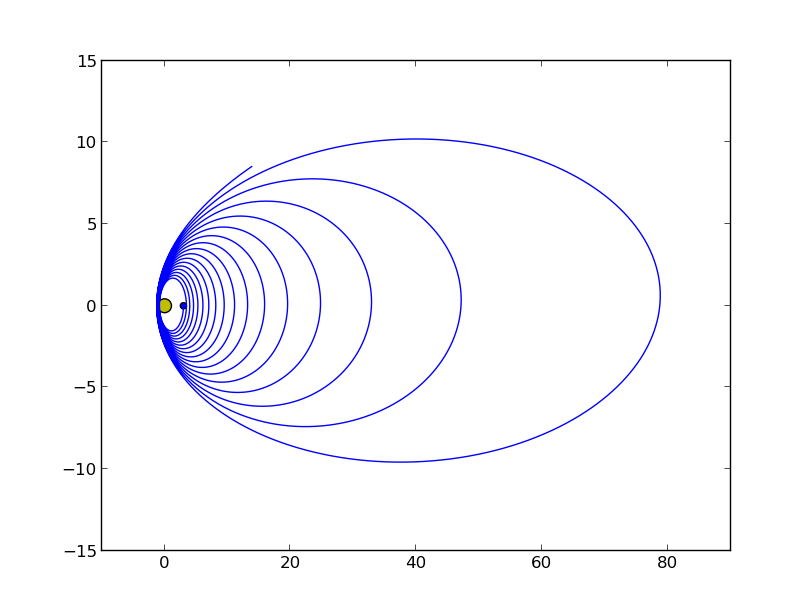
\includegraphics[scale = 0.4]{elipsoide.png}
%\captionof{solution approchée : trajectoires elliptiques}
\label{elipse}
\end{minipage} \hfill
\begin{minipage}{0.45\textwidth}
Pour obtenir une solution approchée à cette équation différentielle nous utilisons l'une des méthodes décrites dans la partie 1. La figure ~\ref{elipse} montre par exemple le résultat obtenue par la méthode d'Euler avec les conditions initales suivantes :
\begin{itemize}
\item Corps A : $(m_{A} = 100, x_{A} = 0, y_{A} = 0)$
\item Corps B : $(m_{B} = 1, x_{B} = 3, y_{B} = 0, \dot x_{B} = 0, \dot y_{B} = -3)$
\end{itemize}
En théorie, les solutions doivent correspondre à des coniques (cercles, ellipse, hyperboles et paraboles). En pratique nous n'obtenons pas de bonnes approximations pour ces coniques (ellipse dans l'exemple). En effet, plus on avance dans le temps plus ces trajectoires divergent de la conique initiale.
\end{minipage}


Ce comportement erroné est dûe à l'imprécision des méthodes de calcul, notamment le choix du pas. Nous avons remarqués dans nos test que pour toutes les méthodes, ce comportement se produit même en diminuant le pas.
\subsection{Problème à trois corps}
Nous considérons maintenant un troisième corps C de masse négligeable devant A et B. Le centre de gravité du système composé de A, B et C est situé au centre de A. De plus le corps B est supposé en rotation circulaire autour de A. Nous cherchons à obtenir la trajectoire de C.
On applique le pricipe fondamental de la dynamique à nouveau et on obtient l'équation différentielle suivante :
\begin{center}
$Y^{'} = f(t,Y) = \begin{pmatrix}
  \dot x_{C} \\
  \dot y_{C} \\
   \frac{Gm_{A}(x_{A} - x_{C})}{((x_{A} - x_{C})^{2} + (y_{A} - y_{C})^{2})^{\frac{3}{2}}} + \frac{Gm_{B}(cos(t) - x_{C})}{((cos(t) - x_{C})^{2} + (sin(t) - y_{C})^{2})^{\frac{3}{2}}}\\
   \frac{Gm_{A}(y_{A} - y_{C})}{((x_{A} - x_{C})^{2} + (y_{A} - y_{C})^{2})^{\frac{3}{2}}} + \frac{Gm_{B}(sin(t) - y_{C})}{((cos(t) - x_{C})^{2} + (sin(t) - y_{C})^{2})^{\frac{3}{2}}}\\
\end{pmatrix}$
\end{center}

Afin de bien visualer la trajectoire du point C, nous allons tracer le résultat obtenu à partir de l'une des méthodes de résolution dans le référentiel en rotation lié à B, en effectuant un changement de base. Dans ce référentiel, seul le point C est en mouvement.

La figure~\ref{cmp} représente les trajectoires de deux points C1 et C2 correspondant aux états initiaux suivants :
\begin{itemize}
\item C1 : $(x_{C1} = -0.75, y_{C1} = 0, \dot x_{C1} = 1, \dot y_{C1} = 1)$
\item C2 : $(x_{C2} = -0.7, y_{C2} = 0, \dot x_{C2} = 1, \dot y_{C2} = 1)$
\end{itemize}
On remarque que pour ces deux points dont les états initiaux sont presque confondues, les trajectoires commencent à diverger infiniment au bout d'un certain temps. On en déduit que le problème des trois corps est chaotique, c'est à dire qu'il est imprévisible et que sa solution dépend des conditions initiales.
\begin{figure}[h]
\centering
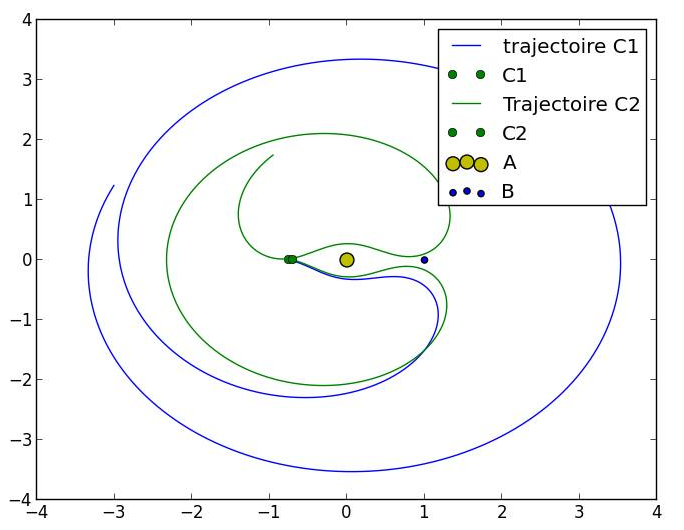
\includegraphics[scale = 0.4]{comparaison.png}
\caption{comparaison de deux trajectoires}
\label{cmp}
\end{figure}





